\def\year{2022}\relax
%File: formatting-instructions-latex-2022.tex
%release 2022.1
\documentclass[letterpaper]{article} % DO NOT CHANGE THIS
\usepackage{aaai22}  % DO NOT CHANGE THIS
\usepackage{times}  % DO NOT CHANGE THIS
\usepackage{helvet}  % DO NOT CHANGE THIS
\usepackage{courier}  % DO NOT CHANGE THIS
\usepackage[hyphens]{url}  % DO NOT CHANGE THIS
\usepackage{graphicx} % DO NOT CHANGE THIS
\urlstyle{rm} % DO NOT CHANGE THIS
\def\UrlFont{\rm}  % DO NOT CHANGE THIS
\usepackage{natbib}  % DO NOT CHANGE THIS AND DO NOT ADD ANY OPTIONS TO IT
\usepackage{caption} % DO NOT CHANGE THIS AND DO NOT ADD ANY OPTIONS TO IT
\DeclareCaptionStyle{ruled}{labelfont=normalfont,labelsep=colon,strut=off} % DO NOT CHANGE THIS
\frenchspacing  % DO NOT CHANGE THIS
\setlength{\pdfpagewidth}{8.5in}  % DO NOT CHANGE THIS
\setlength{\pdfpageheight}{11in}  % DO NOT CHANGE THIS
%
% These are recommended to typeset algorithms but not required. See the subsubsection on algorithms. Remove them if you don't have algorithms in your paper.
\usepackage{algorithm}
\usepackage{algorithmic}

%
% These are are recommended to typeset listings but not required. See the subsubsection on listing. Remove this block if you don't have listings in your paper.
\usepackage{newfloat}
\usepackage{listings}
\usepackage{multirow}
\usepackage{hhline}
\usepackage{amsmath}
\usepackage{amsfonts}
\usepackage{dsfont}
\usepackage{amsthm}
\usepackage{amssymb}
\usepackage{booktabs}
\usepackage{xcolor}

\lstset{%
	basicstyle={\footnotesize\ttfamily},% footnotesize acceptable for monospace
	numbers=left,numberstyle=\footnotesize,xleftmargin=2em,% show line numbers, remove this entire line if you don't want the numbers.
	aboveskip=0pt,belowskip=0pt,%
	showstringspaces=false,tabsize=2,breaklines=true}
\floatstyle{ruled}
\newfloat{listing}{tb}{lst}{}
\floatname{listing}{Listing}
%
%\nocopyright
%
% PDF Info Is REQUIRED.
% For /Title, write your title in Mixed Case.
% Don't use accents or commands. Retain the parentheses.
% For /Author, add all authors within the parentheses,
% separated by commas. No accents, special characters
% or commands are allowed.
% Keep the /TemplateVersion tag as is
\pdfinfo{
/Title (Hybrid recurrent model for time series with inclusion of external weak signals)
/Author (Etienne David, Jean Bellot, Sylvain Le Corff)
/TemplateVersion (2022.1)
}

% DISALLOWED PACKAGES
% \usepackage{authblk} -- This package is specifically forbidden
% \usepackage{balance} -- This package is specifically forbidden
% \usepackage{color (if used in text)
% \usepackage{CJK} -- This package is specifically forbidden
% \usepackage{float} -- This package is specifically forbidden
% \usepackage{flushend} -- This package is specifically forbidden
% \usepackage{fontenc} -- This package is specifically forbidden
% \usepackage{fullpage} -- This package is specifically forbidden
% \usepackage{geometry} -- This package is specifically forbidden
% \usepackage{grffile} -- This package is specifically forbidden
% \usepackage{hyperref} -- This package is specifically forbidden
% \usepackage{navigator} -- This package is specifically forbidden
% (or any other package that embeds links such as navigator or hyperref)
% \indentfirst} -- This package is specifically forbidden
% \layout} -- This package is specifically forbidden
% \multicol} -- This package is specifically forbidden
% \nameref} -- This package is specifically forbidden
% \usepackage{savetrees} -- This package is specifically forbidden
% \usepackage{setspace} -- This package is specifically forbidden
% \usepackage{stfloats} -- This package is specifically forbidden
% \usepackage{tabu} -- This package is specifically forbidden
% \usepackage{titlesec} -- This package is specifically forbidden
% \usepackage{tocbibind} -- This package is specifically forbidden
% \usepackage{ulem} -- This package is specifically forbidden
% \usepackage{wrapfig} -- This package is specifically forbidden
% DISALLOWED COMMANDS
% \nocopyright -- Your paper will not be published if you use this command
% \addtolength -- This command may not be used
% \balance -- This command may not be used
% \baselinestretch -- Your paper will not be published if you use this command
% \clearpage -- No page breaks of any kind may be used for the final version of your paper
% \columnsep -- This command may not be used
% \newpage -- No page breaks of any kind may be used for the final version of your paper
% \pagebreak -- No page breaks of any kind may be used for the final version of your paperr
% \pagestyle -- This command may not be used
% \tiny -- This is not an acceptable font size.
% \vspace{- -- No negative value may be used in proximity of a caption, figure, table, section, subsection, subsubsection, or reference
% \vskip{- -- No negative value may be used to alter spacing above or below a caption, figure, table, section, subsection, subsubsection, or reference

\setcounter{secnumdepth}{0} %May be changed to 1 or 2 if section numbers are desired.

% The file aaai22.sty is the style file for AAAI Press
% proceedings, working notes, and technical reports.
%

% Title

% Your title must be in mixed case, not sentence case.
% That means all verbs (including short verbs like be, is, using,and go),
% nouns, adverbs, adjectives should be capitalized, including both words in hyphenated terms, while
% articles, conjunctions, and prepositions are lower case unless they
% directly follow a colon or long dash
\title{Hybrid Recurrent Model With External Weak Signals}
\author{
    %Authors
    % All authors must be in the same font size and format.
    Etienne David,\textsuperscript{\rm 1,\rm 2}\\
    Jean Bellot,\textsuperscript{\rm 1}\\
    Sylvain Le Corff\textsuperscript{\rm 2}\\
}
\affiliations{
    %Afiliations
    \textsuperscript{\rm 1}Heuritech, Paris\\
    \textsuperscript{\rm 2}Samovar, T\'el\'ecom SudParis, d\'epartement CITI, TIPIC, Institut Polytechnique de Paris, Palaiseau
    % If you have multiple authors and multiple affiliations
    % use superscripts in text and roman font to identify them.
    % For example,

    % Sunil Issar, \textsuperscript{\rm 2}
    % J. Scott Penberthy, \textsuperscript{\rm 3}
    % George Ferguson,\textsuperscript{\rm 4}
    % Hans Guesgen, \textsuperscript{\rm 5}.
    % Note that the comma should be placed BEFORE the superscript for optimum readability

    %2275 East Bayshore Road, Suite 160\\
    %Palo Alto, California 94303\\
    % email address must be in roman text type, not monospace or sans serif
    etienne.david@heuritech.com, jean.bellot@heuritech.com, sylvain.le$\_$corff@telecom-sudparis.eu
%
% See more examples next
}

%Example, Single Author, ->> remove \iffalse,\fi and place them surrounding AAAI title to use it
\iffalse
\title{My Publication Title --- Single Author}
\author {
    Author Name
}
\affiliations{
    Affiliation\\
    Affiliation Line 2\\
    name@example.com
}
\fi

\iffalse
%Example, Multiple Authors, ->> remove \iffalse,\fi and place them surrounding AAAI title to use it
\title{My Publication Title --- Multiple Authors}
\author {
    % Authors
    First Author Name,\textsuperscript{\rm 1}
    Second Author Name, \textsuperscript{\rm 2}
    Third Author Name \textsuperscript{\rm 1}
}
\affiliations {
    % Affiliations
    \textsuperscript{\rm 1} Affiliation 1\\
    \textsuperscript{\rm 2} Affiliation 2\\
    firstAuthor@affiliation1.com, secondAuthor@affilation2.com, thirdAuthor@affiliation1.com
}
\fi


% REMOVE THIS: bibentry
% This is only needed to show inline citations in the guidelines document. You should not need it and can safely delete it.
\usepackage{bibentry}
% END REMOVE bibentry


\newcommand{\ts}{y}
\newcommand{\fullts}{{\bf \ts}}
\newcommand{\tspred}{\hat{\ts}}
\newcommand{\lvl}{\hat{l}}
\newcommand{\fulllvl}{{\bf \lvl}}
\newcommand{\seas}{\hat{s}}
\newcommand{\fullseas}{{\bf \seas}}
\newcommand{\lsmooth}{\alpha}
\newcommand{\ssmooth}{\beta}
\newcommand{\lag}{h}
\newcommand{\window}{w}
\newcommand{\etspred}{\hat{y}}
\newcommand{\fulletspred}{{\bf \etspred}}
\newcommand{\tswindow}{{\bf \ts}}
\newcommand{\meants}{\Bar{\ts}}
\newcommand{\rnnwindow}{{\bf \rnn}}
\newcommand{\rnn}{z}
\newcommand{\err}{err}
\newcommand{\errwindow}{{\bf \err}}
\newcommand{\rnnmodel}{\textsc{rnn}}
\newcommand{\etsmodel}{\textsc{ets(n,n,a)}}
\newcommand{\ws}{w}
\newcommand{\fullws}{{\bf \ws}}
\newcommand{\wswindow}{{\bf \ws}}
\newcommand{\concatinput}{x}
\newcommand{\fullconcatinput}{{ \bf \concatinput}}
\newcommand{\numberts}{14000}


\begin{document}


\maketitle



\begin{abstract}
Developing models and algorithms to draw causal inference for time series is a long standing statistical problem. It is crucial for many applications, in particular for fashion or retail industries, to make optimal inventory decision and avoid massive wastes. By tracking thousands of fashion trends on social media with stat-of-the-art computer vision approaches, we propose in this paper, the first study of fashion time series forecasting. Our contribution is  twofold. We first provide the first fashion dataset gathering \numberts\ weekly fashion time series. As influence dynamics are the key of emerging trend detection, we associate with each time series several external weak signals representing behaviors of influencers towards the trend. Secondly, to leverage such a complex and rich dataset, we propose a new hybrid forecasting model. Our approach combines per-time-series parametric models with seasonal components and a global recurrent neural network to include sporadic external signals. This hybrid model provides state-of-the-art results on the fashion dataset, and illustrates the benefit of the contribution of  external weak signals.
\end{abstract}


\section{Introduction}

Multivariate time series forecasting is a widespread statistical problem with  many applications, see for instance \citep{sarkka2013bayesian, douc2014nonlinear, zucchini2017hidden} and the numerous references therein.
 %Due to the diversity of applications and use cases, a multitude of models have been proposed. 
 Parametric generative models allow to provide explainable predictions with statistical guarantees based on a precise modeling of the predictive distributions of new data based on a record of past observations. %The parameters of these models are usually estimated using a sequence of observations of the target time series. 
Calibrating these models, for instance using maximum likelihood inference, often requires a fair amount of tuning to design a time series-specific model to provide  accurate forecasts and sharp confidence intervals.  Depending on the use case, statistical properties of the signal and the available data, many families of models have been proposed for time series.  The exponential smoothing model \citep{RePEc:inm:oropre:v:9:y:1961:i:5:p:673-685} or the ARIMA with the Box-Jenkins approach \citep{box2015time} are for instance very popular parametric linear generative models.  Hidden Markov models (HMM) are also widespread and presuppose that available observations are defined using missing data, possibly lying in a high dimensional state space, describing the dynamical system. This hidden state is assumed to be a Markov chain such that at each time step the received observation is a random function of the corresponding latent data.  Although hidden states are modeled as a Markov chain (or a mixing process)  the observations arising therefrom present a highly complex statistical structure. %Introducing latent hidden states, they assume that the predictive distribution is not unique and constant in time but multiple and lead by the values of the hidden states changing during time. 
 In various applications where signals exhibit non-stationarities such as trends and seasonality, classical HMM are not adapted. However, \citep{touron2017modeling}  recently proposed seasonal HMM, assuming that transition probabilities between the states, as well as the emission distributions, are not constant in time but evolve in a periodic manner. Strong consistency results were established in \citep{touron2019consistency} and Expectation Maximization based numerical experiments were proposed.
Altough thes works provide promising results, HMM are computationally expensive to train and are not yet well studied for sequences with thousands of components with a seasonal behavior.
 
 %However, for a large part of applications, parametric generative approaches show limitation to capture  complexity. Accurate candidates can be found with latent data models.  

%During the past decades, forecasting applications have taken a totally new proportion. 
In many fields, single or few time series have become thousands of sequences with complex statistical structures. In this new context, classical time series specific statistical models show limitations when dealing with numerous heterogeneous data. Recurrent neural networks and recent sequence to sequence deep learning architectures offer very appealing numerical alternatives thanks to their capability of leveraging any kind of heterogeneous multivariate data, see for instance \citep{ hochreiter1997long,vaswani2017attention, salinas2020deepar, li2019enhancing, lim2019temporal}. %In the past decades, with the impressive results of deep neural networks (DNN) in vision or language, some time series forecasting applications have been proposed. 
Significant improvements have been achieved with Reccurent Neural Network and its Long Short-Term Memory (LSTM) or Gated Recurrent Unit (GRU)  declinations \citep{8614252}. 
A good example is the DeepAR model \citep{salinas2020deepar}. Based on a LSTM architecture, it can predict accurate probability distributions of the future of a sequence. More recently, applications using the Transformer model have been proposed  \citep{li2019enhancing}. A direct concurrent of the DeepAR model can be found with the Temporal Fusion Transformers (TFT) approach \citep{lim2019temporal}.  Unfortunately, they suffer from two main weaknesses. Firstly, many of them are "black-boxes"  as the final forecast usually does not come with a statistical guarantee  although a few recent works focused on measuring uncertainty in recurrent neural networks, see  \cite{martin2020monte}. Secondly, without a fine prepossessing and well chosen hyper-parameters, these methods could lead to poor results and are often outperformed by traditional statistical parametric models, see \cite{makridakis2018m4}.

In this paper, we consider  new time series forecasting application referred to as {\em fashion trends prediction}. Based on a cutting-edge image recognition technology, we built the first fashion dataset containing \numberts\ sequences representing the apparition of fashion trends on social media per week from 01-01-2015 to 01-01-2019. Our fashion time series has very appealing properties: they have all the same length, same seasonality, no missing value and the absence of sparse time series even for niche trends. The originality of our dataset come from the fact that additional external weak signals can be introduced. With our fashion expertise, we detected several groups of fashion users with a high influence power. Analysing their specific behaviours on social medias, we add to each time series, 4 external weak signals representing the same fashion trends but on a sub-category of users. We call them weak signals because they are often alerts or events that are too sparse, or too incomplete to allow on their own an accurate estimation of their impact on the prediction of the target signal. With this totally new application, we aim at showing a model able to deal with our large fashion dataset, leverage our complex external weak signals and finally provide the most accurate forecasts.
 
Recurrent neural network seems to be the perfect candidate to tackle our forecasting problem due to their capability of leveraging external data.  Recently, hybrid models combining DNN architectures with widespread statistical models to deal with seasonality and trends have been proposed, see for instance  \citep{zhang2003time,jianwei2019novel,bandara2020lstm}. The approach providing the most striking results was proposed in  \citep{smyl2020hybrid} in the context of the M4 forecasting competition \citep{makridakis2020m4}.  Given a large dataset, a per-time-series multiplicative exponential smoothing model is introduced to estimate simple but fundamental components for each time series and compute a first prediction. Then a global recurrent neural network is trained on the entire dataset to correct errors of the previous exponential smoothing models. %With this process, the hybrid approach succeeds at mixing strengths of both model families: robustness of the time series specific parametric models and the power of neural network at learn complex dynamics on large dataset. 
However, the hybrid model has not been designed to deal with external signals even if it include a neural network.

Following this work, we present in this paper a new hyrbid recurrent model for time series forecasting with inclusion of external weak signals. %We design a more general hybrid framework including the original multiplicative model and a new additive one. 
Our approach enriches existing hybrd models  by incorporating an unobserved regime switching feature to account for the need neural network based correction. In order to leverage external signals, we modify the hybrid framework to allow the regime shift and the  global error-corrector neural network to deal with external data. By adding our fashion external weak signals in our proposed framework, we show the real potential of the hybrid approach: a global neural network, able to leverage large amount of data, deal with any kind of external weak signals, learn context and finally correct weaknesses and errors of the parametric models.

The paper is organized as follow. Section~\ref{sec:hybrid} describes our hybrid framework which consists of an exponential smoothing model and a recurrent neural network combining the target sequences with external weak signals. Then, we present our new fashion dataset in Section~\ref{sec:dataset}. Section~\ref{sec:exp} describes our results and comparisons with several benchmarks. Finally, we conclude our paper and detail research perspectives in Section~\ref{sec:discussion}.


\section{Hybrid model with external signals}
\label{sec:hybrid}
We introduce a new hybrid approach for time series forecasting  composed of two parts: an additive exponential smoothing (ETS) per time series and a global RNN. We use a per time series statistical model to learn local behaviour and to normalize sequences before feeding them to the neural network. Then, we use a recurrent neural network and weak signals to correct the predictions provided by the ETS.

Consider $N\geqslant 1$ time series. For all $1\leqslant n \leqslant N$ and $1\leqslant t \leqslant T$, let $\ts_t^n$ be the value of the $n$-th sequence at time $t$ and  $\fullts^n = \{\ts_t^n\}_{1\leqslant t \leqslant T}$ be all the values of this sequence.   The objective of this paper is to propose a model to  forecast all time series in a given time frame  $\lag \in \mathbb{N}$, i.e. we aim at sampling $\{\ts^n_{t+1:t+\lag}\}_{1\leqslant n \leqslant N}$ based on $\{\ts^n_{1:t}\}_{1\leqslant n \leqslant N}$.

%It is assumed that for all $1\leqslant n \leqslant N$, $\fullts^n$ is a seasonal time series with a season equal to $m \in \mathbb{N}$, $m$ equals 4 for quarterly, 12 for monthly or 52 for weekly time series. However, no restriction in term of scale and noise distributions are assumed in the generative law of each time series.

\subsection{Per time series statistical model}
%The first step in our additive hybrid model is to consider, for each time series, an exponential smoothing  statistical model.
The time-series-specific models compute, for each sequence, two components,  level  and  seasonality. For all $1\leqslant n \leqslant N$ and $0\leqslant t \leqslant T$, let $\lvl_t^n$ be the value of the $n$-th level component at time $t$ and  $\fulllvl^n = \{\lvl_t^n\}_{0\leqslant t \leqslant T}$ be all the values of this level component. For all $1\leqslant n \leqslant N$ and $-m+1\leqslant t \leqslant T$, let $\seas_t^n$ be the value of the $n$-th seasonality component at time $t$ and  $\fullseas^n = \{\seas_t^n\}_{-m+1\leqslant t \leqslant T}$ be all the values of this season component. $m \in \mathbb{N}$ is the seasonality length (4 for quarterly, 12 for monthly or 52 for weekly time series). Given the sequence $\fullts^n$, the two components  $\fulllvl^n$ and $\fullseas^n$ are computed using exponential smoothing.
For all $1\leqslant n \leqslant N$, let $\Theta^n = \{\alpha^n, \gamma^n,\{\seas_t^n\}_{-m+1\leqslant t \leqslant 0}\}$ be the parameters of the $n$-th sequence with $\lsmooth^n$ and $\ssmooth^n$ the positive smoothing parameters and $\{\seas_t^n\}_{-m+1\leqslant t \leqslant 0}$ the $m$ first seasonality terms. We initialize the first level with $\lvl^n_{0} = \sum_{t = 1}^m \ts^n_{t}/m$ and, for all $1\leqslant n \leqslant N$ and $1\leqslant t \leqslant T$,
\begin{align*}
    \lvl^n_{t} &= \lsmooth^n (\ts^n_t - \seas^n_{t-m}) + (1- \lsmooth^n)\lvl^n_{t-1}\,, \\
    \seas^n_t &= \ssmooth^n (\ts^n_t - \lvl^n_{t-1}) + (1 - \ssmooth^n)\seas^n_{t-1}\,. 
\end{align*}

For all $n \in \{1,\ldots,N\}$, given the level component $\fulllvl^n$, the seasonality component $\fullseas^n$ and the forecast horizon $\lag \in \mathbb{N}$, the exponential smoothing forecast $\{\etspred^{ets,n}_{T+1:T+\lag|T}\}_{1\leqslant n \leqslant N}$ is, for all $i \in \{1,\ldots,\lag\}$,
$$
\etspred^{ets,n}_{T+i|T} = \lvl^n_T + \seas^n_{T+i-m(k+1)}\,,
$$
where $k = \lfloor(i-1)/m\rfloor$. 

%For this first stage, we decided to use an additive exponential smoothing for many reasons: firstly, it is easily understandable and it is pretty robust for any kind of sequences. 

This statistical model offers a fine approach to normalize and deseasonnalize the sequences. In addition, with its two recurrent equations only, it is simple to code and incorporate in a larger framework using deep learning model and GPUs. However, other statistical methods could have been used as the basis of our hybrid approach. For example, S. Smyl created his hybrid model with a multiplicative exponential smoothing model instead of the additive form. At the end, The main complexity is in the next stage: succeed in training a global RNN to understand all the per-time-series statistical models and correct their mistakes.

\subsection{Regime switching error-corrector recurrent model}

Then we train a global RNN on all sequences to compute a correction of the first statistical prediction. We motivate this choice for two reasons. Firstly, pure machine learning methods achieve relatively poor results in time series forecasting. Turning a full forecasting task into a correcting task largely simplifies the RNN goals. Secondly, neural network needs a thorough data pre-processing and classical pre-processing methods are not really suited for time-series. With our collection of exponential smoothing models, we propose a fine way to normalize and deseasonalize the RNN inputs and outputs. %We describe bellow how we design a RNN able to understand the first exponential smoothing models and estimate a correction of their forecasting errors.

Let $\window \in \mathbb{N}$ be the window size, usually this input window is equal to the forecast horizon $\window = \lag$. Consider the following  normalized, deseasonalized and rescaled sequence $\rnnwindow^n_T = \{\rnn^{n}_{T-\window+i|T}\}_{1\leqslant i \leqslant w}$, where, for all $1\leqslant n \leqslant N$ and $1\leqslant i \leqslant w$, 
$$
\rnn^{n,T}_{T-w+i|T} = \frac{\ts^n_{T-w+i} - \lvl^n_T - \seas^n_{T-w+i}}{\meants^n_T}\,,
$$
where $ \meants^n_T = \sum_{i = 1}^{w}  \ts^n_{T-w+i}/w$. This new input is used to correct the exponential smoothing prediction. %Write, for all $1\leqslant n \leqslant N$ and all $i \in \{1,\ldots,H\}$, $\err^{n,T}_{T+i|T} = \ts^n_{T+i} - \etspred^{ets,n}_{T+i|T}$. 
Consider then a recurrent neural network denoted by RNN which aims at predicting the exponential smoothing error. Given $\rnnwindow^n_T$, the proposed model is given, for all $1\leqslant n \leqslant N$ and all $i \in \{1,\ldots,\lag\}$, by
$$
\ts^n_{T+i}  = \etspred^{ets,n}_{T+i|T} +  U^n_T\times\meants^n_T\times \rnnmodel(\rnnwindow^n_T)_{T+i} + \varepsilon^n_{T+i}\,,%\\
%  &= \lvl^n_T + \seas^n_{T+i-m(k+1)} +  U^n_T\times\meants^n_T\times \rnnmodel(\rnnwindow^n_T)_{T+i} + \varepsilon^n_{T+i}\,,
$$
where $\{\varepsilon^n_{T+i}\}_{i\leqslant 1}$ are independent random variables with \textcolor{red}{specify here the right distribution} and $U^n_T$ an unobserved regime switching Bernoulli random variable. The random variable $U^n_T$ allows to provide RNN corrections only when ETS prediction is not sharp enough \textcolor{red}{Show in appendix cases where ETS alone is enough and cases where correction is required}. The law of $U^n_T$ is parameterized by a Feed Forward Neural Network (FFNN) with input \textcolor{red}{complete here}.
%$$
%\ts^n_{T+i} = \rnnmodel(\rnnwindow^n_T)_{T+i} = \frac{\hat{\err}^{n,T}_{T+i|T}}{\meants^n_T}
%$$
%Finally, for all $1\leqslant n \leqslant N$, the  final forecast of the model is $\{\tspred^{n}_{T+1:T+\lag|T}\}_{1\leqslant n \leqslant N}$, where, for all $i \in \{1,\ldots,\lag\}$ :
%\begin{align*}
%\tspred^n_{T+i|T}  &= \etspred^{ets,n}_{T+i|T} +  \meants^n_T\times \rnnmodel(\rnnwindow^n_T)_{T+i}\,,\\
%  &= \lvl^n_T + \seas^n_{T+i-m(k+1)} + \hat{\err}^{n,T}_{T+i|T}\,.
%\end{align*}

\subsection{Weak signal}

Using a time-series-specific statistical model, the hybrid network achieves striking accuracy on single sequences. Then, the shared recurrent neural network relies on the strength of machine learning methods at leveraging a huge quantities of heterogeneous data.
In addition to the $N$ target time series, we consider $K \times N$ external sequences indexed from $0$ to $T$. For all $1\leqslant n \leqslant N$, $1\leqslant k \leqslant K$ and  $1\leqslant t \leqslant T$, let $\ws^{n,k}_t$ be the value of the $k$-th external sequence at time $t$ linked to the sequence $\fullts^n$. We note $\fullws^n = \{\{\ws_t^{n,k}\}_{1\leqslant t \leqslant T}\}_{1\leqslant k \leqslant K}$ all the values of the family of weak signals linked to the $n$-th sequence. In addition, let $\fullws^n_T = \{\{\ws_{T-w+i}^{n,k}\}_{1\leqslant i \leqslant \window}\}_{1\leqslant k \leqslant K}$ be only the last $\window$ terms of the family. Concatenating $ \rnnwindow^n_T$ and $\fullws^n_T$, we define a new input for our RNN,   
\begin{align*}
\fullconcatinput^n_T &= \{\concatinput^n_{T-w+i|T}\}_{1\leqslant i \leqslant w}\,, \\
&= \{\rnn^n_{T-w+i|T}, \ws^{n,1}_{T-w+i},...,\ws^{n,K}_{T-w+i}\}_{1\leqslant i \leqslant w}\,.
\end{align*}
Finally, for all $1\leqslant n \leqslant N$ and for all $i \in \{1,\ldots,\lag\}$ our final model becomes:
%$$
%\tspred^n_{T+i|T} 
%= \etspred^{ets,n}_{T+i|T} +  \rnnmodel(\fullconcatinput^n_T)_{T+i} \times \meants^n_T
%$$
\begin{equation}
\label{eq:full:model}
\ts^n_{T+i}  = \etspred^{ets,n}_{T+i|T} +  U^n_T\times\meants^n_T\times \rnnmodel(\fullconcatinput^n_T)_{T+i} + \varepsilon^n_{T+i}\,,
\end{equation}
\textcolor{red}{specify here the right distribution for $U$ (depends on the weak signal or no)}. The complete architecture is displayed in Figure~\ref{fig:architecture}.

\begin{figure}
  \centering
    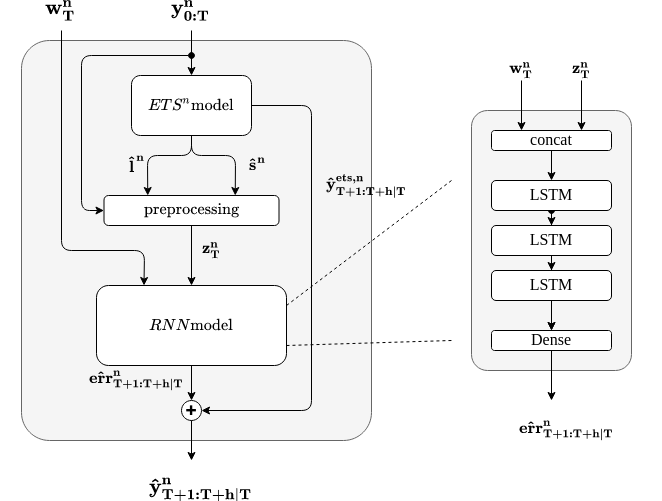
\includegraphics[width=0.8\linewidth]{figure/hybrid_model_archi.png}
  \caption{Hybrid model with weak signals architecture.}
\label{fig:architecture}
\end{figure}

As $U^n_T$ is not observed, the loglikelihood of the observations cannot be written explicitly to train the model. Therefore we use Fisher's identity to compute the score function and write a gradient ascent algorithm to estimate simultaneously the weights of the RNN and of the FFNN denoted by $\theta$. The score is
\begin{multline*}
\nabla_\theta \log p_\theta(\ts^n_{T+1:T+h}|\ts^n_{1:T})
\\ = \mathbb{E}\left[\nabla_\theta \log p_\theta(\ts^n_{T+1:T+h},U_T^n|\ts^n_{1:T})\middle|\ts^n_{1:T+h}\right]\,,
\end{multline*}
where the joint likelihood $p_\theta(\ts^n_{T+1:T+h},U_T^n|\ts^n_{1:T}) = p_\theta(U_T^n|\ts^n_{1:T})p_\theta(\ts^n_{T+1:T+h}|U_T^n,\ts^n_{1:T})$ is given by \eqref{eq:full:model} and the expectation is under the posterior distribution of $U_T^n$ given $\ts^n_{1:T+h}$  \textcolor{red}{details to add in appendix}. \textcolor{red}{Assume that $\theta_p$ is the current value for the weights of the FFNN and the RNN and write $\omega_p^n = \mathbb{P}_{\theta_p}(U_T^n = 1|\ts^n_{1:T+h})$. Note that
$$
\omega_p^n \propto \mathbb{P}_{\theta_p}(U_T^n = 1|\ts^n_{1:T})p_{\theta_p}(\ts^n_{T+1:T+h}|U_T^n=1,\ts^n_{1:T})\,.
$$
Then,
\begin{multline*}
\nabla_\theta \log p_\theta(\ts^n_{T+1:T+h}|\ts^n_{1:T}) = \omega_p^n\nabla_\theta \log p_\theta(\ts^n_{T+1:T+h},U_T^n=1|\ts^n_{1:T})\\
+ (1-\omega_p^n)\nabla_\theta \log p_\theta(\ts^n_{T+1:T+h},U_T^n=0|\ts^n_{1:T})\,.
\end{multline*}
The loss function is then given by
\begin{multline*}
\theta\mapsto - \omega_p^n \log p_\theta(\ts^n_{T+1:T+h},U_T^n=1|\ts^n_{1:T})\\
- (1-\omega_p^n) \log p_\theta(\ts^n_{T+1:T+h},U_T^n=0|\ts^n_{1:T})\,,
\end{multline*} 
where no gradient is computed on $\omega_p^n$. In both terms, $\log p_\theta(U_T^n=0|\ts^n_{1:T})$ and $\log p_\theta(U_T^n=0|\ts^n_{1:T})$ are simply given by the output of the FFNN.  Choices for the model.
\begin{itemize}
\item In the case where the  $\varepsilon^n_{T+i}$ are Gaussian and independent, up to an additive constant
$$
\log p_\theta(\ts^n_{T+1:T+h}|U_T^n=0,\ts^n_{1:T}) = -c\sum_{i=1}^{h}(\ts^n_{T+i}  - \etspred^{ets,n}_{T+i|T})^2
$$
and
\begin{multline*}
\log p_\theta(\ts^n_{T+1:T+h}|U_T^n=1,\ts^n_{1:T})\\
 = -c\sum_{i=1}^{h}(\ts^n_{T+i}  - \etspred^{ets,n}_{T+i|T} - \meants^n_T\times \rnnmodel(\fullconcatinput^n_T)_{T+i})^2\,.
\end{multline*}
Choice of $c$ ?
\item In the case where the  $\varepsilon^n_{T+i}$ are Laplace and independent, up to an additive constant
$$
\log p_\theta(\ts^n_{T+1:T+h}|U_T^n=0,\ts^n_{1:T}) = -c\sum_{i=1}^{h}|\ts^n_{T+i}  - \etspred^{ets,n}_{T+i|T}|
$$
and
\begin{multline*}
\log p_\theta(\ts^n_{T+1:T+h}|U_T^n=1,\ts^n_{1:T})\\
 = -c\sum_{i=1}^{h}|\ts^n_{T+i}  - \etspred^{ets,n}_{T+i|T} - \meants^n_T\times \rnnmodel(\fullconcatinput^n_T)_{T+i}|\,.
\end{multline*}
Choice of $c$ ?
\end{itemize}}

\section{Fashion dataset with external weak signals}
\label{sec:dataset}
In image of language processing, there are available reference datasets covering varieties of applications. However, for time series forecasting, there is a lack of large, rich and public datasets where neural network approaches can express their potential. With the M4 and M5 competitions, we can find large amounts of data but they show several limitation. For example the M4 dataset does not propose external signals in addition to the time series. Conversely, the M5 one does so but like other sales datasets \citep{C.Favorita}, it includes a majority of sporadic time series that do not allow the application of some kinds of models\citep{makridakis2020m5}. With this paper, we aim at widening the set of available datasets for time series forecasting with the first fashion dataset including external weak signals.

Heuritech is the first company to adopt a data-intensive approach  for the fashion forecasting. It analyzes every day images shared on social networks thanks to a high throughput computer vision systems. Aggregating detected clothes by trends, we create thousands of time series with the same good properties: same weekly seasonality, shared behaviours and the same length: from 2015-01-05 to 2020-09-01. Each time series is normalized in order to remove social networks biases and their values lie between 0 and 1. The proposed fashion dataset contains $\numberts$ anonymized fashion trends for men and women, on 9 differents categories and 5 geozones. An overview of it can be found in table 1.



\begin{table*}
  \caption{Fashion time series overview. For each couple geozone/category, we give the number of female and male trends (Female/Male)}
  \label{sample-table}
  \centering
  \resizebox{\textwidth}{!}{
  \begin{tabular}{lllllllllll}
    \toprule
    &  Top  & Pants & Short & Skirt & Dress & Coat & Shoes & Color & Texture &  \\
    \midrule
     United States & 587/290 & 195/158  & 64/37 & 38/- & 38/- & 271/218 & 439/114 & 59/59 & 129/103\\
     Europe & 587/290 &  195/158& 64/37 & 38/- & 38/- & 271/218 & 439/114 & 59/59 & 135/111\\
     Japan &  587/290 & 193/158 & 64/37 & 38/- &  37/- & 271/218 &  429/114 & 59/59 &  124/98\\
     China &  586/290 & 195/158 & 64/37 & 38/- &  37/- & 271/218 &  433/114 & 59/59 &  128/113\\
     Brazil &  587/290 & 195/158 & 64/37 & 38/- &  38/- & 271/218 & 439/114 & 59/59 & 136/110\\
     \midrule
     Total & 2934/1450 & 973/790 & 320/185 & 190/- & 188/- & 1355/1090 & 2179/570 & 295/294 & 652/535 & \numberts\\
    \bottomrule
  \end{tabular}
  }
\end{table*}



In addition to this large dataset we design for each sequence several weak signals :
\begin{itemize}
    \item Firstly, we create a specific fashion-oriented panel of micro-influencers. In theoretical fashion dynamics \citep{rogersdiffusion}, different categories of adopters adopt a trend in succession, resulting in several adoption waves. With this specific panel, we aim at detecting the first waves announcing emerging trends or the collapse of other ones. By analyzing images shared by this specific panel on social medias, we create a first weak signal named \textit{fashion-forwards} for each of the previous trends.
    \item for the other weak signals, we analyzed only a specific part of social media users depending of the number of followers. With three thresholds we create the following external signals : \textit{followers-low}, \textit{followers-mid} and \textit{followers-high}. The first one represents users with few followers, the second one is made of users with a moderate amount of followers and the last one gathers superstar and users of any fields with thousands of influencers. Again, the motivation here is to detect behaviour gaps between this three segments that could announce bigger changes in the main signal.
\end{itemize}

At the end, we have for each trends 4 linked weak signals representing this trends on a specific panel of social media users. These extra signals are frequently sparse for micro trends and they often lack of interest for common fashion trends. However on several examples, they are fundamental to detect the future fashion evolution. 

As an example, an impressive emerging fashion trend is represented in figure 2. The graph shows the evolution of one of our shoes trends on social media and its linked \textit{fashion-forward} weak signal. During the first 3 years, common users and our panel of mode-influencers share the same behaviour. The trend start to boom in the mainstream people during the first month of 2018. However, we can detect early signals in the fashion-forward panel at the end of 2017. Early adopters started to change there behaviour and show more frequently the trend on social media. With fashion influence dynamics, the new tendency spreads to every part of social media users and more generally on the society. Finally, after a pick reached at the end of 2018 for our fashion-influencers, a regular decrease appear. They leave gradually the old trend to focus more on the latest or propose new ones. 

\begin{figure}
  \centering
    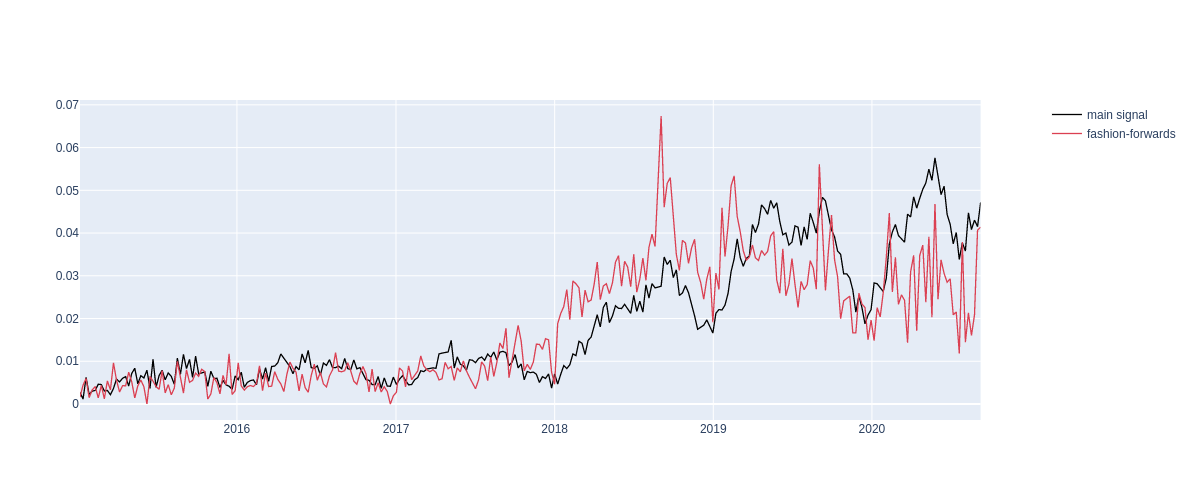
\includegraphics[width=1.\linewidth]{figure/good_example.png}
  \caption{A shoes trend of our dataset. In black the main signal and in red its associated \textit{fashion-forward} weak signal. The Gap between our two signals in the end of 2017/beginning of 2018 announces the future explosion of the fashion trend.}
\end{figure}



\section{Experimental results}
\label{sec:exp}
In this section, we evaluate how our hybrid framework is able to deal with the fashion dataset and leverage our complex external weak signals. To lead our experience, we keep hide the last year of each time series as our test set. For each method and each time series, based on the first five years of data, we predict the last year and compute our accuracy on it.

\subsection{Training}

To train our hybrid models, we made the choice of don't using the original code of the hybrid method provided during the M4 competition. Indeed, the proposed implementation is difficult to use in a more general framework and it is quite slow because it doesn't enable the use of GPU. Thereby, we propose with this paper, a new version of the hybrid framework, including the original multiplicative model and the new additive one. Our proposed code is developed in Python using the Tensorflow library and it allows the use of a GPU to speed up the training process.

In addition to a more general framework, we add the possibility of doing inference with our new implementation. We design a new process to compute and provide a forecast for a totally  new collection of sequences without retraining the entire hybrid model. Given a new time series, we freeze the weights of the error-corrector recurrent model and we only train the new time-series-specific statistical model linked to the new sequence. It remains the responsibility of the users to provide new sequences sharing same behaviours than the dataset using for the training to keep the same accuracy level.

For more details about the general hybrid training, a complete description of the training process can be found in the M4 hybrid model paper or in an interesting application of the method on electric load forecasting, see \citep{dudek2020hybrid}.

\subsection{Benchmarks, hybrid models and Metrics}

As benchmarks, we chose several well-known statistical methods and a full Machine Learning (ML) model. For the statistical part, using the R package "forecast", we compute for each time series a prediction with the following methods: \textit{snaive}, \textit{stlm}, \textit{thetam}, \textit{tbats} and \textit{auto.arima}. \textit{Snaive} forecasts are only the repetition of the last same past period. \textit{stlm} approach use a multiplicative decomposition and models the seasonality adjusted time series with an exponenantial smoothing model. \textit{Thetam} model decompose the original signal in $\theta$-lines, forecast each one separately and recompose them to produce the final forecast. \textit{tbats} is a powerful statistical model using a trigonometrical seasonality modelization. The last one \textit{auto.arima} is the R implementation of ARIMA model with an automatic selection of the best parameters. For the full ML method, we train a global Long-Short Term Memory (\textit{lstm}) neural network on all our dataset. Against these models, we propose two versions of the hybrid approach without the external weak signal. The first one is the original multiplicative form of the hybrid model that we name \textit{hybrid-mul}. The second one is the additive variant described in Section~\ref{sec:hybrid} and we named it \textit{hybrid-add}. To reach a higher accuracy level we propose at the end an ensembling (\textit{ensembling} of our two hybrid approaches using the FFORMA method created during the M4 competition, see \citep{fforma} . 

Finally, to evaluate the power of our external signals and the capacity of our hybrid models to leverage them, we propose for our two approaches a version with the external weak signals. We name them respectively \textit{hybrid-mul-ws} for the multiplicative version and \textit{hybrid-add-ws} for the additive one. As benchmarks we propose the same comparison with our previous full ML model \textit{lstm} with a version including weak signals \textit{lstm-ws}.


To compare the different methods, we use the same metrics as in the M4 competition: the Mean Absolute Scaled Error (MASE), the Symmetric Mean Absolute Percentage Error (SMAPE) and the final M4 competition metric, the Overall Weighted Average (OWA) of the SMAPE and the MASE. 


$$
MASE = \frac{\frac{1}{h}\sum_{i=1}^h |Y_i - \hat{Y}_i| }{\frac{1}{T-m}\sum_{i=1}^{T-m} |Y_i - Y_{i-m}|} \quad
SMAPE = \frac{1}{h} \sum_{i=1}^h \frac{2|Y_i - \hat{Y}_i|}{|Y_i| + |\hat{Y}_i|}
$$

$$
OWA = \frac{1}{2}(\frac{MASE}{MASE_{snaive}} + \frac{SMAPE}{SMAPE_{snaive}})
$$

\subsection{Heuritech Fashion dataset results}

In a first place, Table 2 shows the final accuracy of the statistical models, the LSTM model and our 2 hybrid models without external data. Even without the weak signals, our 2 hybrid approaches largely outperform the statistical references. The multiplicative model show the best accuracy with a OWA equal to 0.875. We can note that the additive model slightly under-performs the traditional multiplicative one on average. This doesn't show a weakness of the additive version but more that a large part of our dataset is more-suited for multiplicative modelization. At the end, the strength of training both methods, additive and multiplicative, is in the final porposed ensembling \textit{ensembling} that combines the two approaches with the FForma ensembling.

In a second place, Table 3 shows the evaluation of our 4 trained hybrid models: the 2 previous ones without weak signals, and our 2 full hybrid models with weak signals. We present also the accuracy of a simple LSTM model with and without weak signals. We can show the impressive improvement due to our external signals. Again, the multiplicative method achieves the best accuracy with OWA metric equal to 0.860. We propose like previously, an ensembling mixing our two full hybrid models with weak signals and it reach the high level of accuracy with an OWA equal to 0.849.

In a third place, table 4 presents the result of our inference process. We split our dataset in five equal parts of 2800 sequences and hide the last year for each trends. Then, like a cross validation, we train a model on 4 parts and compute its accuracy on the last one on the last year. The model never saw the last part so we use our inference process to compute predictions. With a permutation of the parts, we can repeat the process and train 5 models, each trained on a specific pool of 4 parts and tested on the remaining part of the dataset. For each hybrid model (additive/multiplicative with and without weak signals) Table 4 shows the average accuracy and the Standard Deviation of the 5 trained hybrid models. We can see that our inference process achieve really accurate results and practically the same that our hybrid models trained on the entire dataset. These results prove that, even without having seen a sequence during the training, if the time series share same behaviours that the training sample, our hybrid approaches can perfectly compute accurate predictions. Furthermore, the Standard Deviation is really low for all our metrics. This result shows that our hybrid framework is robust and reach constant accuracy level on large dataset.


Finally, with our results, we can make two interesting conclusions: 
\begin{itemize}
    \item Firstly, the hybird modeling is a really promising framework. By mixing the performance of local parametric models and a global DNN, our two versions clearly outperform traditional statistical methods. Furthermore, this framework is totally suited for dealing with external signals. With a fine pre-processing and a well-designed architecture, our two models succeed at leveraging our complex extra data and reach an impressive accuracy levels.
    \item Secondly, our results bring to light the quality of our new Fashion dataset. Even without weak signal, our DNN based model outperforms time series specific model. This show that our dataset is well suited to train complex neural network architectures able to learn information cross sequences. With the addition of our weak signals, we give a totally new dimension to our fashion dataset. Our results show that our external weak signals hide a complex but usable predictive power by DNN architecture. By making it publicly available, we hope that it will enhance the set of datasets for time series forecasting.
\end{itemize} 


\subsection{Discussion}

\begin{table*}
  \caption{Results summary (Mean/Median) on our Fashion dataset. In a first time, we train our hybrid approaches without our external weak signals.}
  \label{sample-table}
  \centering
  \begin{tabular}{lllllll}
    \toprule
    &  MASE  & MASE-std & SMAPE & SMAPE-std & OWA & OWA-std  \\
    \midrule
     snaive & 0.983/0.936 & 0.33 & 27.68/24.42 & 15.0 & 1./1. & 0.\\
     thetam & 0.924/0.869  & 0.35 & 25.82/22.54  & 14.6 & 0.952/0.915 & 0.26\\
     stlm & 0.893/0.834 & 0.35 & 25.07/21.93  & 14.3 & 0.917/0.895 & 0.21\\
     tbats & 0.886/0.822  & 0.34 &  24.81/21.60 & 14.0 &  0.910/0.882 & 0.22 \\
     lstm & 0.881/0.824 & 0.34 & 24.41/21.56 & 12.81 & 0.895/0.885 & 0.11 \\
     hybrid-add & 0.863/0.812  & 0.32 & 24.17/21.36 & 13.0 & 0.877/0.880 & 0.08 \\
     hybrid-mul & 0.858/0.817 & 0.30 & 24.06/21.30 & 13.0 & 0.876/0.873 & 0.11 \\
     Ensembling & 0.846/0.804 & 0.30 & 23.78/21.07 & 12.9 & 0.864/0.863 & 0.10  \\
    \bottomrule
  \end{tabular}
\end{table*}

\begin{table*}
  \caption{Comparison between our hybrid models without and with our external weak signals, (Mean/Median)}
  \label{sample-table}
  \centering
  \begin{tabular}{lllllll}
    \toprule
    &  MASE  & MASE-std & SMAPE & SMAPE-std & OWA & OWA-std \\
    \midrule
    lstm & 0.881/0.824 & 0.34 & 24.41/21.56 & 12.81 & 0.895/0.885 & 0.11 \\
    lstm-ws & 0.869/0.814 & 0.33 & 24.56/21.33 & 14.40 & 0.890/0.874 & 0.132 \\
     hybrid-add & 0.863/0.812  & 0.32 & 24.17/21.36 & 13.0 & 0.877/0.880 & 0.08 \\
     hybrid-mul & 0.858/0.817 & 0.30 & 24.06/21.30 & 13.0 & 0.876/0.873 & 0.11 \\
     hybrid-add-ws & 0.852/0.807 & 0.30 & 24.03/21.17 & 13.0 & 0.872/0.869 & 0.10 \\
     hybrid-mul-ws & 0.836/0.798 & 0.29 & 23.67/20.87 & 12.9 & 0.860/0.858 & 0.12 \\
     Ensembling & 0.827/0.787 & 0.29 & 23.43/20.63 & 12.8 & 0.849/0.849 & 0.11\\
    \bottomrule
  \end{tabular}
\end{table*}



\begin{table*}
  \caption{Cross-Validation. we split our dataset in 5 equal parts. We train for each hybrid approach, 5 models on 4 specific parts of the dataset and we test them of the remaining parts with our inference process.}
  \label{sample-table}
  \centering
  \begin{tabular}{lllllll}
    \toprule
    &  MASE  & MASE-std & SMAPE & SMAPE-std & OWA & OWA-std \\
    \midrule
     hybrid-add & 0.861  & 0.004 & 24.16 & 0.18 & 0.877 & 0.002 \\
     hybrid-mul & 0.856 & 0.008 & 23.95 & 0.25 & 0.870 & 0.005 \\
     hybrid-add-ws & 0.848 & 0.004 & 24.00 & 0.18 & 0.869 & 0.002 \\
     hybrid-mul-ws & 0.844 & 0.010 & 23.74 & .20 & 0.863 & 0.006 \\
    \bottomrule
  \end{tabular}
\end{table*}




\section{Conclusion}
\label{sec:discussion}
In this paper, we propose the first hybrid model including external weak signals for time series forecasting. We show that hybrid framework is a really promising way. With its extended error-corrector DNN part, it is clearly well-suited for dealing with any kind of external signals in order to correct weaknesses of first parametric models. Furthermore, With our additive version, we show that the hybrid model is not frozen in it original form. Thereby, future research explorations would be to improve its framework with new per-time-series approaches and test new error-corrector DNN part like the recent Transformer model.

With this first contribution, we join the first fashion dataset gathering \numberts\ mode times series and a complex collection of extra signals. We believe that this dataset hide really fine dynamics and interactions where complex models would express their potential. By making it publicly available, we hope that it will enhance the set of datasets for time series forecasting and pave the way for further explorations.

\bibliography{aaai22.bib}

\section{Appendices}

\subsection{RNN architecture and baselines}
\label{section:architectures}

\subsection{Further training details}
\label{section:train_details}

\subsection{Details on the Fashion dataset}
\label{section:dataset_details}

\subsection{Examples from the dataset}
\label{section:examples}

\end{document}